%%
%% Use the options `twocolumn,final' to obtain the final layout
%\documentclass[twocolumn,final]{elsarticle}
\documentclass[review,12pt]{elsarticle}
%\documentclass[final,3p,times]{elsarticle}
\usepackage{framed,multirow}
\usepackage{mathptmx}
\usepackage{epstopdf}
\usepackage{subcaption,graphicx}
%\usepackage{subfigure}% Support for small, `sub' figures and tables
\usepackage{float}
\usepackage{amssymb}
\usepackage{latexsym}
\usepackage{lineno}
\usepackage{url}
\usepackage{xcolor}
\usepackage{mathtools}
\definecolor{newcolor}{rgb}{.8,.349,.1}
\journal{Computer Methods and Progrms in Biomedicine}

\begin{document}

\thispagestyle{empty}

\begin{frontmatter}
\title{False-positive reduction in computer-aided mass detection using mammographic texture analysis and classification}

\author{Jaroslaw Kurek$^{\rm a}$, Sami Dhahbi$^{\rm b}$, Bartosz Swiderski $^{\rm a}$,  Michal Kruk$^{\rm a}$, Walid Barhoumi$^{\rm b}$, Grzegorz Wieczorek$^{\rm a}$, Ezzeddine Zagrouba$^{\rm b}$, Katarzyna Zagrodzka$^{\rm a}$ \\
 $^{a}$The Faculty of Applied Informatics and Mathematics, Warsaw University of Life Sciences, 166 Nowoursynowska Street, 02-787 Warsaw, Poland \\%
 $^{b}${\em{LIMTIC Laboratory, ISI, 2 Street Abou Rayhane Bayrouni, 2080 Ariana, Tunisia}}\\
jaroslaw{\_}kurek@sggw.pl, sami{\_}dhahbi@yahoo.fr, bartosz{\_}swiderski@sggw.pl,  michal{\_}kruk@sggw.pl, walid.barhoumi@enicarthage.rnu.tn, grzegorz{\_}wieczorek@sggw.pl, ezzeddine.zagrouba@fsm.rnu.tn, kasia.zagrodzka92@gmail.com
}
%\maketitle
\begin{abstract}
\textit{Background: } Mammographic mass detection is a challenging problem due to the confusing appearance of some normal tissues that visually look like masses. Current computer-aided detection (CAD) systems for the case of mammographic masses suffer from high false positive rates, resulting in unnecessary biopsies and overlook by radiologists.\\
\textit{Methods:} This paper copes with this problem and proposes a framework to reduce false positive masses detected by CAD. 
 %Indeed, we investigated several feature extraction methods, including two commonly used methods for mammogram descriptions (gray level co-occurrence matrix and fractal analysis) and three methods applied for the first time for mammogram analysis (Hilbert’s image representation, Kolmogorov-Smirnov distance and maximum subregion descriptors).
  To avoid the error induced by the segmentation step, we proposed a segmentation-free framework with particular attention to improve feature extraction and classification steps.
We investigated for the first time in mammogram analysis, Hilbert's image representation, Kolmogorov-Smirnov distance and maximum subregion descriptors.
  Then, a feature selection step is performed to select the most discriminative features. Moreover, we considered several classifiers such as Random Forest, Support Vector Machine and Decision Tree to distinguish between normal tissues and masses.\\
\textit{Results:} The proposed method is evaluated on a large database composed of 10168 suspicious regions extracted from the DDSM database. The normal cases were previously detected by a CAD system, which makes this database more challenging. Experimental results prove the efficiency of the suggested method for false-positive reduction in mammographic mass detection.
\\
\textit{Conclusions:}  In summary, gray level texture features could be used to reduce false-positive cases in CAD systems for breast cancer diagnosis.

\end{abstract}

\begin{keyword}
mammography \sep false-positive reduction \sep breast cancer diagnosis \sep Hilbert’s image representation


\end{keyword}

\end{frontmatter}

\section{Introduction}

Breast cancer is the most dangerous cancer among women in both developed and developing countries. According to Globocan statistics, breast cancer is the most diagnosed female cancer that affected 1.67 million new cases (25\% of all female cancers) worldwide in 2012 \citep{Ferlay2012}. It is also the leading cause of cancer deaths among women that killed 522,000 women (14.7\% of cancer-related deaths) \citep{Dhahbi2015}. Breast cancer is arising from cells of the breast that develops locally in the breast and metastasizes to the lymph nodes and internal organs. Even though some studies pointed out several risk factors of having breast cancer such as genetics and tobacco, the cause of cell metastasize is not clearly known. This makes early prevention of breast cancer not possible. Thus, early detection is considered as the cornerstone in breast cancer treatment. A breast cancer detected at early stage is easy to handle, whereas late detection decreases treatment options and increases mortality rates. Unfortunately, traditional detection methods such as palpable breast examination or clinical women request (after pain) usually detect cancers at non-recoverable stages. Screening programs are applied to cope with this issue: women with higher risk (such as old women) but with no clinical symptoms are examined. The best cost-effective tool for breast cancer detection is currently screening mammography. It can detect breast abnormalities at an early stage when they are not detectable by a woman or doctor, what increases very significantly the chance of cure \citep{Jotwani2009}. For instance, several developed countries established systematic nation-wide screening mammography programs for early breast cancer detection: each woman over 50 years undergoes a mammography examination every two (or three) years.  These programs helped in reducing the mortality rate of breast cancer \citep{Nelson2009,Hofvind2009}.

However, mammography interpretation is a difficult and error prone task, even for skilled radiologists, mainly due to the subtle signs of breast abnormalities and the overlapping dense fibro-glandular tissue. Misinterpretation of mammograms leads to false positives and/or false negatives. False positives-taking normal tissue for abnormalities-result in high recall rates with unnecessary treatments (such as invasive biopsies). False negatives-missing a cancer abnormality-complicate treatment options and threaten patient life. Due to the huge amount of screening mammograms to be analyzed and the limited number of radiologists, double reading by a second radiologist, which is usually performed for diagnostic mammograms, is not feasible in screening programs. A cost-effective alternative to human double reading is the use of Computer Aided Detection systems (CAD), which can replace the second reader and alert the radiologist to suspicious regions. These systems have improved the detection rates of breast abnormalities such as micro-calcification and masses. Given that the detection of masses is much more challenging because some normal tissues may look visually similar to masses and can be taken for abnormalities, the aim of this work is to reduce mass false positives produced by CAD systems. Indeed, the main drawback of CAD systems for masses is false positives, which may increase biopsy rates. Besides, given the low rate of cancer occurrence in screening programs, radiologists may over-look CAD outputs that contain many suspicious regions.  Hence, a posterior step of reduction of false positive rates in CAD systems is crucial to reduce unnecessary follow-up treatments and to ensure radiologist’s acceptance.

Several studies have focused on reducing false positives for masses. Hence, given suspicious regions detected by a CAD system, false positive reduction (FPR) methods aim to classify these regions as normal or abnormal.  A first class of methods aimed to include information from the current mammogram or other views. For instance, \cite{Vallez2014} included a breast density classification step prior to lesion detection so that to improve the detection results.
 \cite{Li2015} used a bilateral similarity analysis to combine information from right and left breast views. \cite{Tan2014} proposed a score fusion to combine detection results of medio-lateral oblique (MLO) view and cranio-caudal (CC) view.
  A second class of methods  solved the pattern recognition problem of distinguishing between normal tissues and masses in three steps: lesion segmentation, feature extraction, and binary classification.
For instance, \cite{Junior2013} used a spatial approach of diversity indexes to describe patterns detected in previously segmented regions and a SVM classifier to classify regions into masses and non-masses. \cite{Liu2015} used  adaptive region growing and narrow band based active contour  for mammographic masses segmentation,   gray level co-occurrence matrix (GLCM) and complete local binary patterns (CLBP) for the  description of the segmented lesions, and  SVM for classification.
\cite{Sampaio2015} performed masses segmentation based on micro-genetic algorithm. Then,  Local binary patterns and SVM were used to classify the suspicious regions.
However, the segmentation of mammographic masses is a very difficult task and error-prone. Therefore, some authors proposed to omit the segmentation step and to compute the feature vector directly from the ROI.  For instance, \cite{Dhahbi2015} proposed a multiscale texture analysis method for false positive reduction based on curvelet moments. Curvelet transform was first performed on region of interest (ROI). Moment statistics (mean, variance, kurtosis and skewness) were then computed from each curvelet band and were input into a k-nearest-neighbor (kNN) classifier. A feature selection step was also included to select the most relevant curvelet moments. \cite{Zyout2015} reduced false positive of mass detection based on multiscale textural feature extraction, particle swarm optimization and support vector machines (SVM) classification.  \cite{Hussain2014} introduces a method for false positive reduction based on Weber law descriptor (WLD) and SVM classification.
{\cite{Jiang2015,Liu2014} used SIFT features to describe mammographic ROIS for scalable mammogram retrieval.


Our main motivation in this work is to improve the performance of mammographic masses detection through false-positive reduction. To avoid the error induced by the segmentation step and to take into account the texture around the lesion, we proposed a segmentation-free framework with particular attention to improve  feature extraction and classification steps.  Hence,   we propose five different feature extraction methods to describe mammographic regions. The first method extracts 23 features based on Hilbert’s image representation. The second method uses fractal texture analysis to extract 36 features. The third set is composed of 38 Kolmogorov-Smirnov distances. The fourth set consists of 15 features corresponding to statistics from the gray level co-occurrence matrix (GLCM). The last method is based on K-S statistic and Minkowsky approach to compute 10 features corresponding to maximum sub-region descriptors. To the best of our knowledge, Hilbert’s image representation, Kolmogorov-Smirnov distances and maximum sub-region descriptors are introduced for the first time for mammographic masses analysis and false positive reduction. Once the 122 features are computed, we performed a sequential feature selection method to choose the most discriminative subset. For the classification step, even though the SVM classifier is the most common classifier for mammographic masses classification,   other classifiers could yield better results.
Therefore, we investigated three different  classification methods: SVM, decision tree and random forest.
The main contributions of the paper are as follows:
\begin{enumerate}
 \item Effective representation of mammographic masses through Hilbert’s image representation, Kolmogorov-Smirnov distances and maximum sub-region descriptors.
  \item  Combination of the proposed three feature sets with two other commonly used sets: fractal texture features and gray level co-occurrence matrix statistics.
  \item Selection of the most discriminative features for masses description.
  \item Investigation of three different classification methods.
  \item Experimental evaluation of the proposed framework in a large and challenging database.
\end{enumerate}

The rest of this paper is organized as follows. Sections 2 describes the used mammograms in the experiments. Section 3 presents the feature extraction methods we used to generate diagnostic features. Section 4  recalls the feature selection method. Section 5 is devoted to numerical experiments. Conclusions are stated in Section 6.

\section{Database}
In the experiments, we used mammograms from the Digital Database for Screening Mammography (DDSM) \citep{Heath1998}, which is the largest public mammogram dataset. DDSM includes 2604 cases, each case is composed of four mammograms corresponding to Cranial-Caudal (CC) and Medio-Lateral-Oblique (MLO) views for right and left breasts. The dataset includes the ground truth of each mammogram, mainly its diagnostic result (normal, benign or malignant) and the location of existing lesions.  Since the whole mammographic image comprises the pectoral muscle and the background with a lot of noise, features were computed on a limited ROI that contains the prospective abnormality \citep{Dhahbi2015}.

\begin{figure}
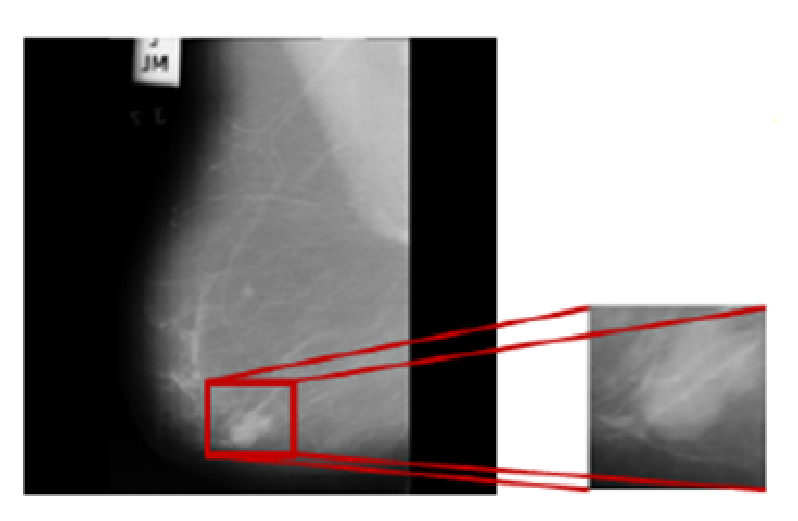
\includegraphics[scale=0.7]{images/ROINEW.eps}
\caption{Example of region of interest (ROI) extraction}
\label{fig:ROI}
\end{figure}

Thus, cropping a region of interest removes the unwanted parts. This is an important step to extract and focus on appropriate part of mammography image.
In the experiments, a large database of a total number of 10168 ROIs has been used:
\begin{enumerate}
  \item Normal tissue – 8254 ROIs,
  \item Benign lesion – 862 ROIs,
  \item Malignant lesion - 1052 ROIs.
\end{enumerate}

For the abnormal cases (benign and malignant),  a manual cropping was performed based on the information provided in the ground truth.
Thus, ROIs depicting masses are simply rectangular area centred on the coordinates of the lesion provided in the ground truth (Figure 1).
 The normal regions  used in this study correspond to false positive masses provided by a previous CAD system from healthy cases \citep{Jiang2015}.
Compared to common databases in which normal cases are manually extracted by authors  from the healthy tissues, the dataset we used in this study is more realistic and more challenging \citep{Jiang2015}.
Besides, since the false reduction step does not aim to distinguish malignant from benign cases, we merged benign lesions and malignant ones into abnormal cases. Finally, we obtained the two following classes:
\begin{enumerate}
  \item Normal tissue – 8254 ROIs
  \item Abnormal tissue – 1914 ROIs
\end{enumerate}
In the experiments, all the ROIs were resized to $256 \times 256$ pixels.
Figure 2 illustrates examples of ROIs used in the experiments.
\begin{figure}
\center
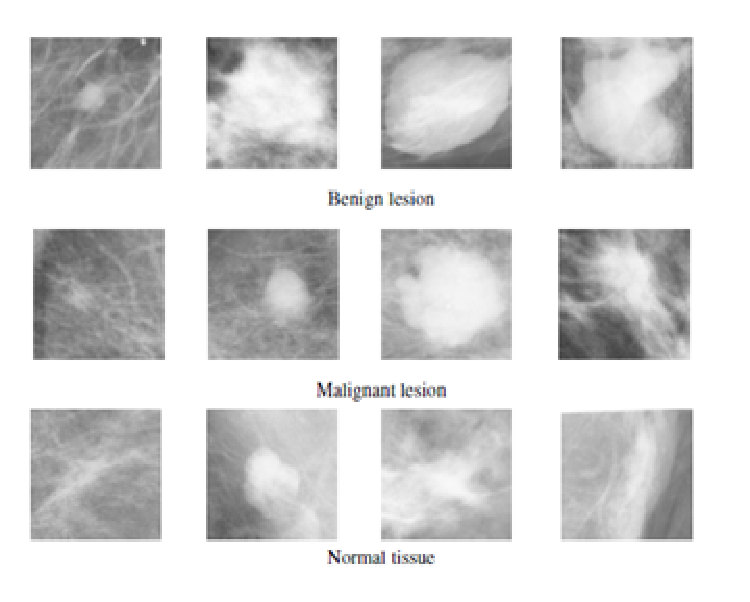
\includegraphics[scale=0.7]{images/ROIsamples.eps}
\caption{Sample of used ROIs from the DDSM database}
\label{fig:ROIsamples}
\end{figure}

\section{Generation of diagnostic features}
Our whole database of masses consists of totally 10168 cropped images (ROI). This set has been divided into normal tissues and abnormal tissues (1914 ROI's), based on accurate diagnosis performed manually by doctors. Our approach now is to generate features, which differentiate between the two classes (normal/abnormal tissue) the best.

During the manual analysis of the images of normal and abnormal tissues, it is easy to notice that the main differences among pectoral muscles are connected with the shape, size, granulites, texture, colour and intensity of the images associated with different states of tissues. In our approach to this problem, we will base on the features referred to characteristics of chaotic image, changes in the features distribution, co-occurrence haralick's matrix, fractal dimension and regular statistical features.

On the basis of all extracted ROI’s, we generated in total 122 potential diagnostic features for binary classification. Features have been extracted based on every grayscale image from the whole database (10168 grayscale images). The dataset of potential diagnostic features consists of the following groups:

\begin{itemize}
\item features generated based on Hilbert’s image representation (35 features) .
\item features generated based on coaxial rigs image representation and Kolmogorov-Smirnov distance approach (14 features).
\item features generated based on Maximum regions descriptors (6 features).
\item features generated based on forest fire modelling (2 features).
\item features generated based on the gray-level co-occurrence matrix - GLCM (4 features).
\item features generated based on box-counting fractal dimension (9 features).
\item features generated based on segmentation-based fractal texture analysis (36 features).
\item features generated based on 4-level wavelet packet decomposition (16 features).
\end{itemize}

\subsection{Hilbert’s image representation}\label{R3.1}

A Hilbert curve or  Hilbert space-filling curve is a continuous fractal space-filling
curve, first described by the German mathematician David Hilbert in 1891. It was one variant of  filling space  with curves discovered by Giuseppe Peano in 1890. The Hilbert's curve (Figure \ref{fig:Hilbert}) appears to have useful characteristics.

Both the true Hilbert curve and its discrete approximations are useful because they provide a mapping between 1D and 2D space that fairly well preserves locality \citep{Jiang2015},\citep{Matlab2015}.

For many extracted features (especially statistical features), where one dimensional matrix (vector) is required as an algorithm input, we should find the best representation of every grayscale image. One of the best 1-dimensional image representation is the application of the Hilbert' curve. One-dimensional matrix is the result of covering discrete Hilbert's transformation mask for the image. Hence, this one dimensional matrix can be treated as a vector and can be a base for any feature extraction algorithm, where one dimensional matrix is strictly required.

\begin{figure}
\center
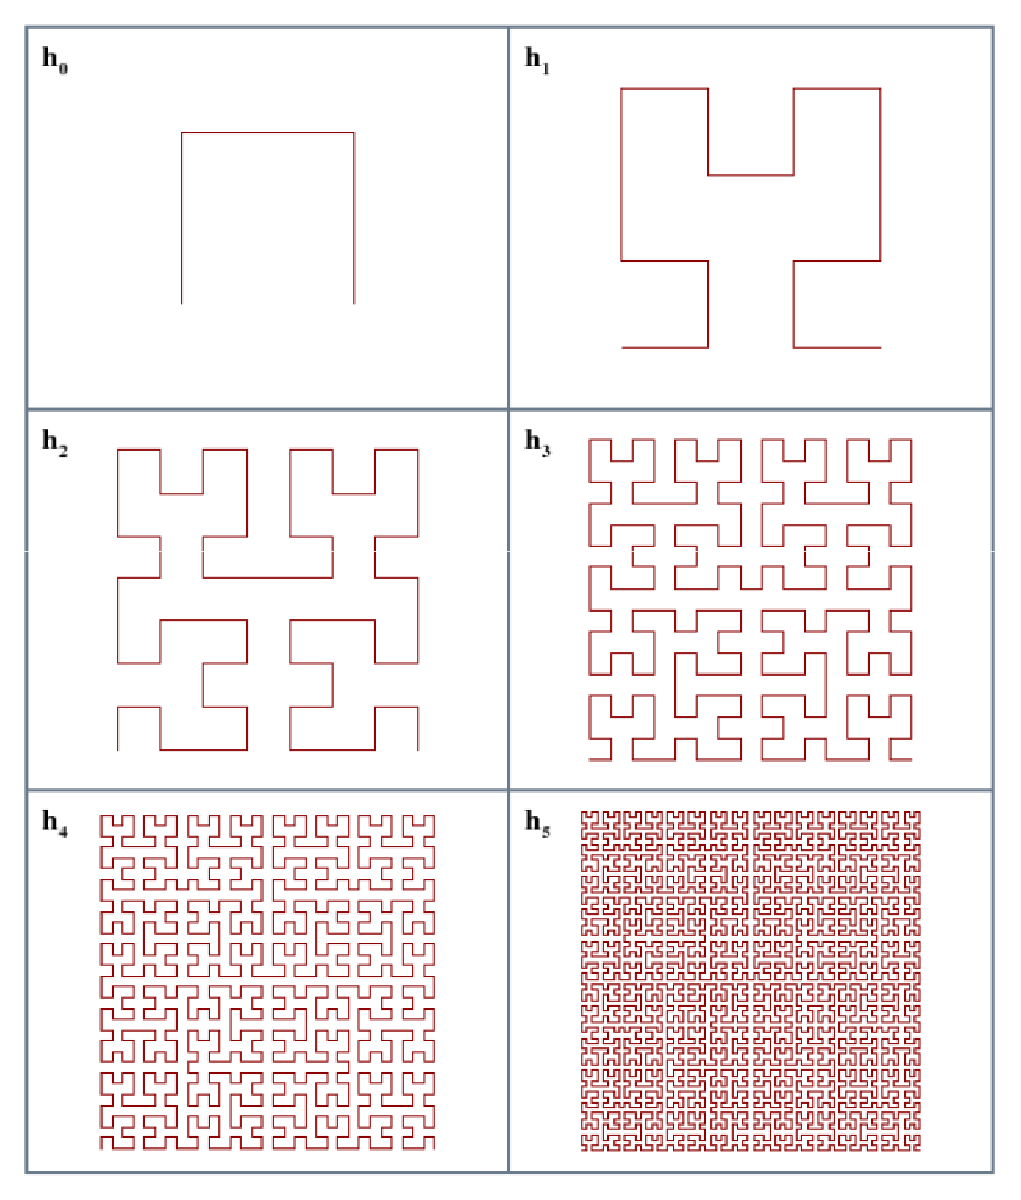
\includegraphics[scale=0.5]{images/Hilbert.eps}
\caption{Example of discrete Hilbert's curve for order 0,1,2,3,4,5, respectively}
\label{fig:Hilbert}
\end{figure}

Let's assume that we have to fill the space with curves and the space has the square size if $n\times m$, where n is the power of 2 e.g. 4, 8, 16, 32. Building the Hilbert's curve of order respectively 0,1,2,3,4,5 is depicted on Figure \ref{fig:Hilbert}. Based on the above assumption, we can generate discrete the Hilbert's curve using the following recursive formula:

\begin{subequations} \label{subeqHilbert}

\begin{equation}
x_{0}=0
\label{subeqHilberta}
\end{equation}

\begin{equation}
y_{0}=0
\label{subeqHilbertb}
\end{equation}

\begin{equation}
\textbf{x}_{n}=\frac{1}{2}\left[
                   \begin{array}{cccc}
                     (y_{n-1}-0.5) & (x_{n-1}-0.5) & (x_{n-1}+0.5) & (-y_{n-1}+0.5) \\
                   \end{array}
                 \right]
\label{subeqHilbertc}
\end{equation}

\begin{equation}
\textbf{y}_{n}=\frac{1}{2}\left[
                   \begin{array}{cccc}
                     (x_{n-1}-0.5) & (y_{n-1}+0.5) & (y_{n-1}+0.5) & (-x_{n-1}-0.5) \\
                   \end{array}
                 \right]
\label{subeqHilbertc}
\end{equation}

\end{subequations}

The advantages of applying the discrete Hilbert's curve for one-dimensional image representation are as follows:
\begin{itemize}
\item mapping between 1D and 2D space fairly well preserves locality
\item when we follow every point of discrete Hilbert's curve, we follow through the image neighbours pixels
\item if $(x,y)$ are the coordinates of a point within the unit square,
and d is the distance along the curve, when it reaches that point, then the points that have nearby d values will also have nearby $(x,y)$ values.
\end{itemize}

In this article, we have constructed the Hilbert's curve order 1024. Then the discrete Hilbert's curve has been mapped to the image. The last stage is the creation of a vector image representation, which consists of all points of the discrete Hilbert's curve. The Matlab code generating the discrete Hilbert's curve is presented below:

\begin{verbatim}
function [x,y] = hilbert(n)
if n<=0
  x=0;
  y=0;
else
  [xo,yo]=hilbert(n-1);
  x=.5*[-.5+yo -.5+xo .5+xo  .5-yo];
  y=.5*[-.5+xo  .5+yo .5+yo -.5-xo];
end
\end{verbatim}


\subsection{Potential 35 features generated based on Hilbert’s image representation}\label{R3.2}

Based on the previously mentioned approach: converting matrix image representation to vector image representation in the form of the discrete Hilbert's curve, the authors have applied many statistic measures where a vector form is required as an input. Some of these statistic measures applied by the authors are presented in Table \ref{TabStatisticalfeatures}. In Total, the authors defined 27 statistic features on the basis of the discrete Hilbert's curve image representation.


}
\begin{table}

\begin{flushleft}
\caption{Some of statistical features based on Hilbert's curve image representation}
\end{flushleft}
{
\begin{tabular}{@{}ll}
\hline
\centering
Name & Equation \\
\hline
Mean & $\mu=\frac{1}{n}\sum_{i=1}^{n}x_{i}$  \\
\cr
Standard deviation & $\sigma=\frac{1}{n}\sqrt{\sum_{i=1}^{n}(x_{i}-\mu)^{2}}$  \\
\cr
Skewness & $S=\frac{1}{n}\sum_{i=1}^{n}(\frac{x_{i}-\mu}{\sigma})^{3}$  \\
\cr
Kurtosis  & $K=\frac{1}{n}\sum_{i=1}^{n}(\frac{x_{i}-\mu}{\sigma})^{4}-3$  \\
\cr
RMS  & $\sqrt{\frac{\sum_{i=1}^{n}|x_{i}|}{n}}$  \\
\cr
Crest factor  & $C=\frac{X_{peak}}{x_{RMS}}$  \\
\hline
\end{tabular}
}
\label{TabStatisticalfeatures}
\end{table}



\subsection{Kolmogorov-Smirnov distance}\label{S3.3}

For some new texture segmentation features generated from the images, the authors have applied Kolmogorov–Smirnov (KS) statistical distance. Some propositions
of applying this statistical measure to the medical image characterization have been already presented in (Demidenko, 2004, Pauwels and Frederix, 2000).

The KS test determines if the samples are drawn from the same underlying continuous population characterized by the cumulative distributions $F(x_{i})$ and $F(x_{j})$ (Figure \ref{fig:KSDistance}). The distance between these two populations is defined by the KS test in the following formula:

\begin{equation}
d_{KS}=max|F(x_{i})-F(x_{j})|
\label{eqKSdistance}
\end{equation}


\begin{figure}
\center
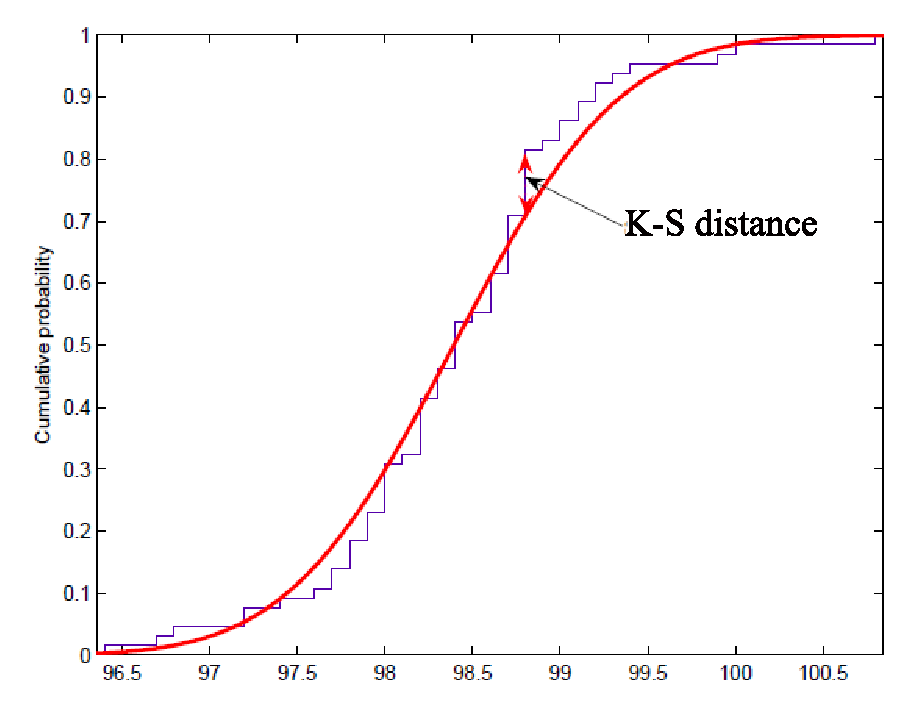
\includegraphics[scale=0.6]{images/KSDistance.eps}
\caption{Example of Kolmogorov - Smirnov test statistic}
\label{fig:KSDistance}
\end{figure}

\subsection{Representation of the neighborhood pixel as a coaxial rings}\label{S3.3}

The aim of this approach is to find features which provide us with the information on the evolution of the 3-dimensional (R,G,B) pixel’s distribution surrounding this point \citep{Kruk2015}. These features should indicate  what is a pace of changes of neighbourhood pixel colours distribution. In our experiment, only the grayscale image has been taken into consideration, hence, we should measure the pace of changes of pixel intensity distribution. To finish the calculation for huge database for every pixel of image in  a reasonable time, only 4 coaxial rings have been constructed, assuming that every coaxial ring should consist of 56 pixels. To compare mentioned distribution, Kolmogorov - Smirnov has been applied. To save a stable distribution, every coaxial rings has the same number of pixels (56 pixels). The representation of the neighborhood pixel in the form of coaxial rings has been depicted on Figure \ref{fig:CoaxialRings}.

\begin{figure}
\center
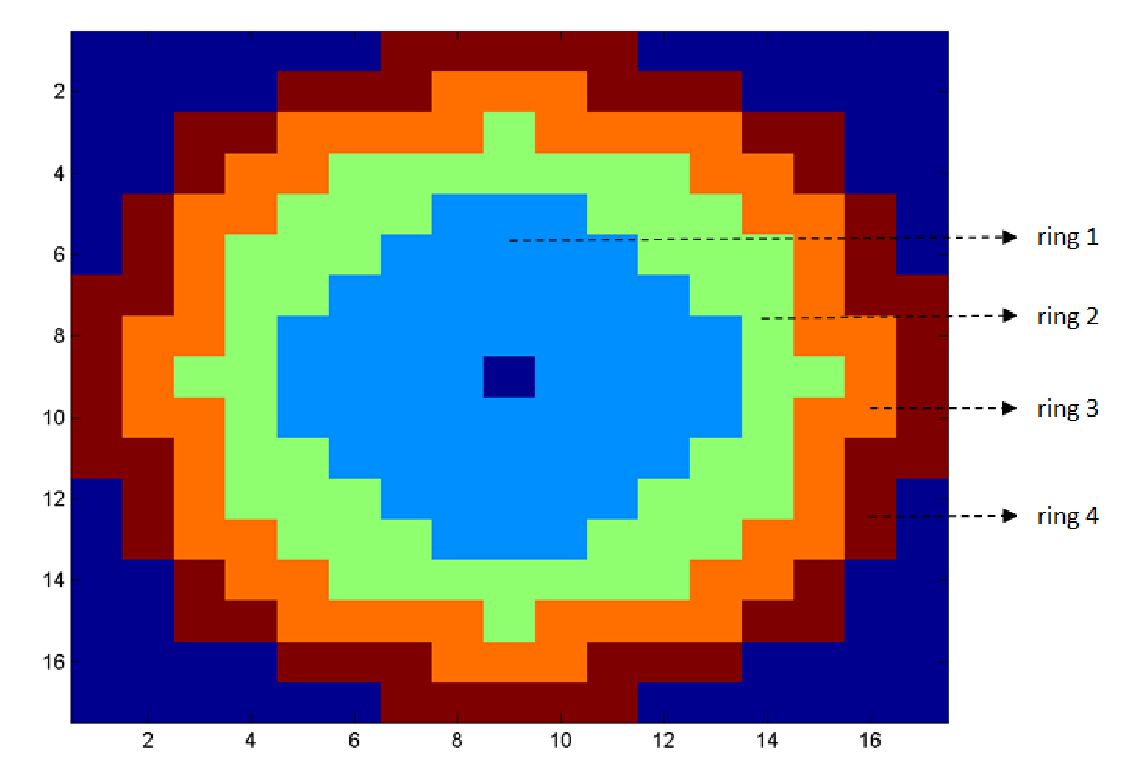
\includegraphics[scale=0.6]{images/CoaxialRing.eps}
\caption{Representation of the neighborhood pixel as a coaxial rings}
\label{fig:CoaxialRings}
\end{figure}

Each analyzed grayscale image was scaled to size $17^{2} \times 17^{2}$ (it means 289 $ \times $ 289), then it has been covered by 17x17 set of coaxial rings. This mechanism has been showed on Figure \ref{fig:17CoaxialRings}.

\begin{figure}
\center
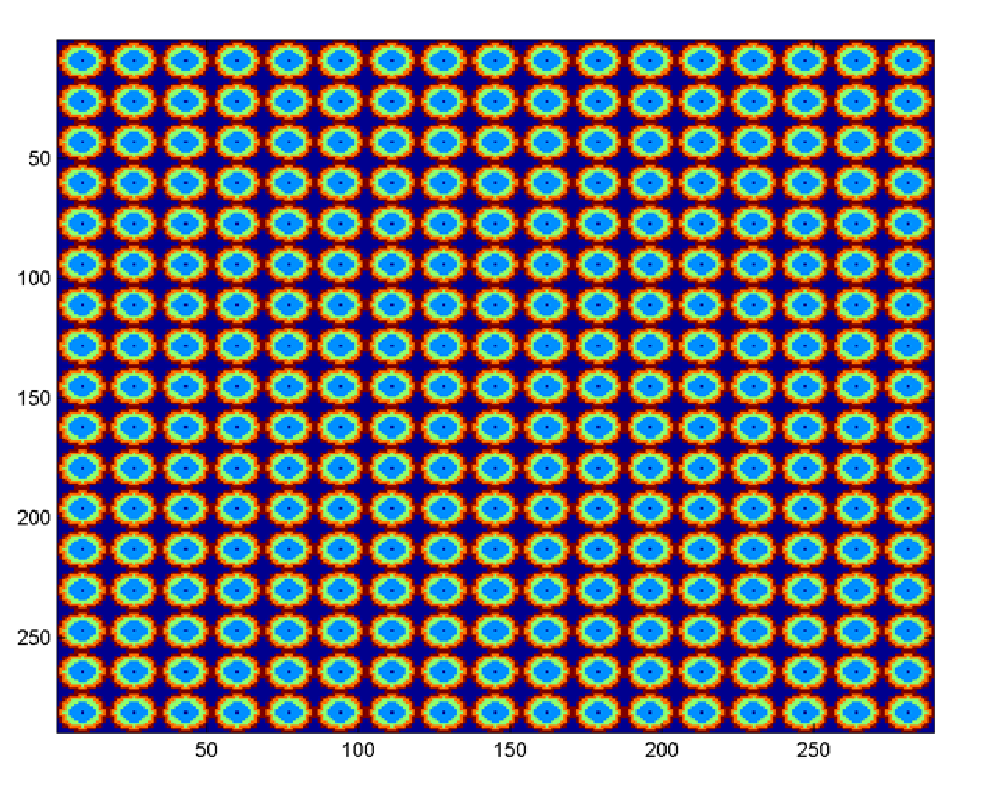
\includegraphics[scale=0.6]{images/17x17rings.eps}
\caption{Representation of image as $17 \times 17$ coaxial rings}
\label{fig:17CoaxialRings}
\end{figure}

For every set of 289 rings, we can compute the KS distances between proper rings as follows (Table \ref{Tab:CalculationKSBEtRings}):

\begin{table}
\caption{Calculation of Kolmogorov-Smirnov distance between coaxial rings}
{
\begin{tabular}{@{}lllll}
\hline
No & $Ring_{i}$ & $Ring_{j}$ & Skipped level ($|i-j|$) & KS \\
\hline
1 & 1 & 2 & 1 & KS1 \\
2 & 1 & 3 & 2 & KS2 \\
3 & 1 & 4 & 3 & KS3 \\
4 & 2 & 4 & 1 & KS4 \\
5 & 2 & 4 & 2 & KS5 \\
6 & 3 & 4 & 1 & KS6 \\
\hline
\end{tabular}
}
\label{Tab:CalculationKSBEtRings}
\end{table}

For all Kolmogorov-Smirnov distances (K-S statistic) in each coaxial ring of the same level, average KS statistic has been calculated. The next step in our approach is the application of the linear regression to the relationship of the average and median KS distance $d_{KS}$ as the function of the level l (Equation \ref{eq:regressionKS}).

\begin{equation}
d_{KS}=\alpha_{0}+\alpha_{1}l+\varepsilon
\label{eq:regressionKS}
\end{equation}

where l denotes skipped level.

Finally, based on coaxial rings image representation and Kolmogorov-Smirnov distance, 14 features have been calculated. These features have been presented in Table \ref{Tab:7features}.

\begin{table}
\caption{Definition of 14 features based on coaxial rings image representation and Kolmogorov-Smirnov distance approach.}
{
\begin{tabular}{@{}lll}
\hline
No & Definition & Description \\
\hline
1 & $d_{KSmean}12$ & mean of KS statistics between rink No. 1 and ring No. 2 \\
\cr
2 & $d_{KSmean}13$ & mean of KS statistics between rink No. 1 and ring No. 3 \\
\cr
3 & $d_{KSmean}14$ & mean of KS statistics between rink No. 1 and ring No. 4 \\
\cr
4 & $\frac{d_{KSmean}13}{d_{KSmean}12}$ & ratio of $d_{KSmean}13$ for $d_{KSmean}12$ \\
\cr
5 & $\frac{d_{KSmean}14}{d_{KSmean}12}$ & ratio of $d_{KSmean}14$ for $d_{KSmean}12$ \\
\cr
6 & $\alpha_{0mean}$ & intercept coefficient of approximation line $d_{KSmean}$ \\
\cr
7 & $\alpha_{1mean}$ & slope coefficient of approximation line $d_{KSmean}$ \\
\cr
8 & $d_{KSmedian}12$ & median of KS statistics between rink No. 1 and ring No. 2 \\
\cr
9 & $d_{KSmedian}13$ & median of KS statistics between rink No. 1 and ring No. 3 \\
\cr
10 & $d_{KSmedian}14$ & median of KS statistics between rink No. 1 and ring No. 4 \\
\cr
11 & $\frac{d_{KSmedian}13}{d_{KSmedian}12}$ & ratio of $d_{KSmedian}13$ for $d_{KSmedian}12$ \\
\cr
12 & $\frac{d_{KSmedian}14}{d_{KSmedian}12}$ & ratio of $d_{KSmedian}14$ for $d_{KSmedian}12$ \\
\cr
13 & $\alpha_{0median}$ & intercept coefficient of approximation line $d_{KSmedian}$ \\
\cr
14 & $\alpha_{1median}$ & slope coefficient of approximation line $d_{KSmedian}$ \\
\hline
\end{tabular}
}
\label{Tab:7features}
\end{table}

\subsection{Maximum regions descriptors}

The main idea is to observe disaggregating the image to smaller consistent subgroups on the basis of the thresholding. We have searched for the level of threshold  from which most subgroups are derived. To obtain the results for dozen thousands images in a reasonable period of time, percentile of pixels intensity has been applied. The result of Maximum Regions Descriptors application has been depicted on Figure \ref{fig:InputMaximumRegionsDescriptors} and \ref{fig:OutputMaximumRegionsDescriptors}.

\begin{figure}
\center
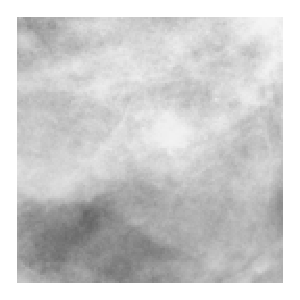
\includegraphics[scale=1.6]{images/InputMaximumRegionsDescriptorsNEW.eps}
\caption{Input image for Maximum Regions Descriptors approach}
\label{fig:InputMaximumRegionsDescriptors}
\end{figure}

\begin{figure}
\center
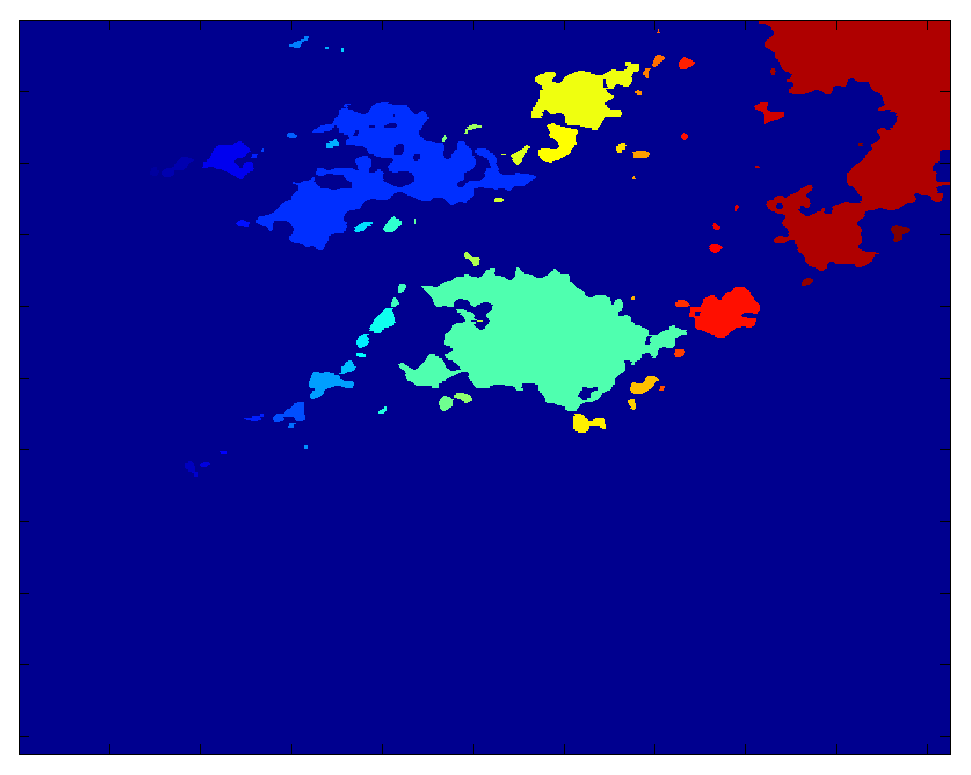
\includegraphics[scale=0.45]{images/OutputMaximumRegionsDescriptorsNEW.eps}
\caption{Output image for Maximum Regions Descriptors approach}
\label{fig:OutputMaximumRegionsDescriptors}
\end{figure}

After finding the threshold associated with disaggregating the image to most subgroups, we can obtain values of our 3 features. These features can be calculated for signs $<$ and $>$, hence we have a total of 6 features (Table \ref{Tab:6features}):

\begin{table}
\caption{Definition of 6 features based on Maximum Regions Descriptors approach.}
{
\begin{tabular}{@{}lll}
\hline
No & Definition & Description \\
\hline
1 & $p_{\geq}$ & associated value of percentile (percentile to intensity: 0.01 → 0 ; 0.99→ 255) for sign ${\geq}$\\
\cr
2 & $q_{\geq}$ & associated percentile (order of quantile) for sign ${\geq}$\\
\cr
3 & $a_{\geq}$ & area of largest subgroup for sign ${\geq}$\\
\hline
\cr
4 & $p_{\leq}$ & associated value of percentile (percentile to intensity:  0.01 → 0 ; 0.99→ 255) for sign ${\leq}$\\
\cr
5& $q_{\leq}$ & associated percentile (order of quantile) for sign ${\leq}$\\
\cr
6 & $a_{\leq}$ & area of largest subgroup for sign ${\leq}$\\
\hline
\end{tabular}
}
\label{Tab:6features}
\end{table}

\subsection{Perlocation coefficients}

The goal in this approach is the use of forest fire modelling to create a potential diagnostic feature based on an image. The idea is based on 9 thresholds (for each decile) of a an image. For every result of thresholding we start setting fire to the forest and then measure the duration of the fire (number of iterations). The fire can be spread only on thresholded area. The authors have applied 8 neighborhood pixels.

The results of stages of the described process are depicted on the figures \ref{fig:inputfire}, \ref{fig:thresholdingfire}, \ref{fig:setingfire}, \ref{fig:firesresult} are depicted results of stages of described process.

\begin{figure}
\center
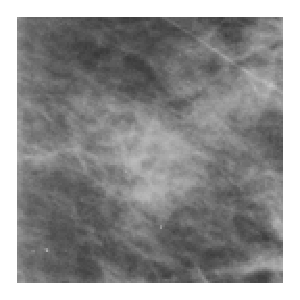
\includegraphics[scale=1.75]{images/input_fire_NEW.eps}
\caption{Image input of forest fire modelling approach}
\label{fig:inputfire}
\end{figure}

\begin{figure}
\center
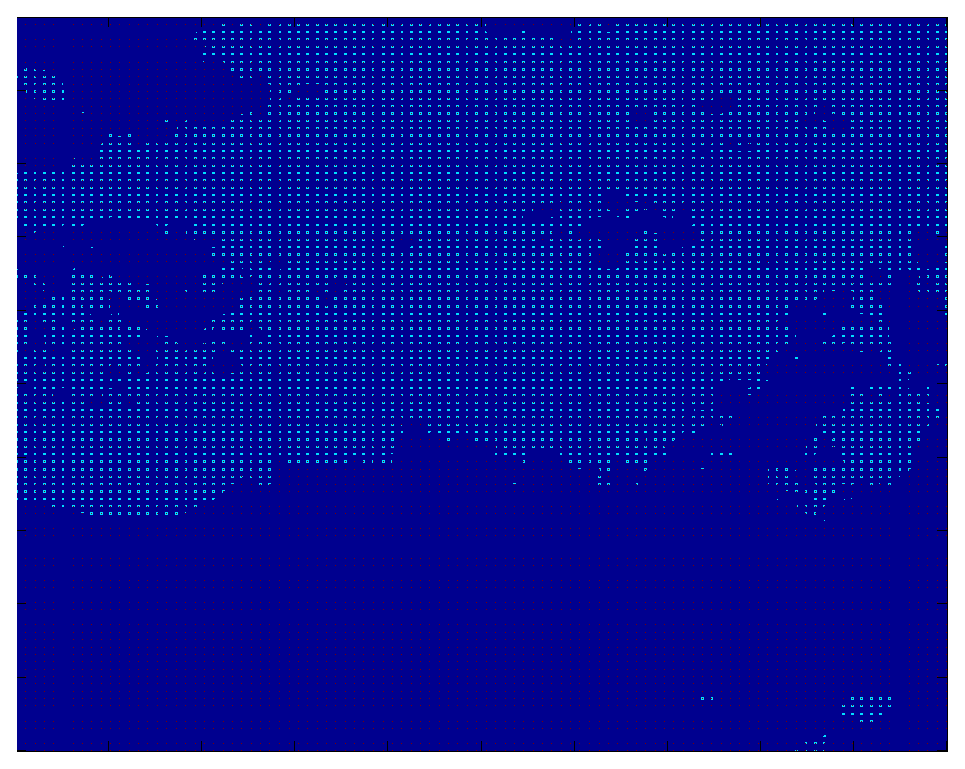
\includegraphics[scale=0.5]{images/seting_fire_NEW.eps}
\caption{Setting fire to the forest}
\label{fig:thresholdingfire}
\end{figure}

\begin{figure}
\center
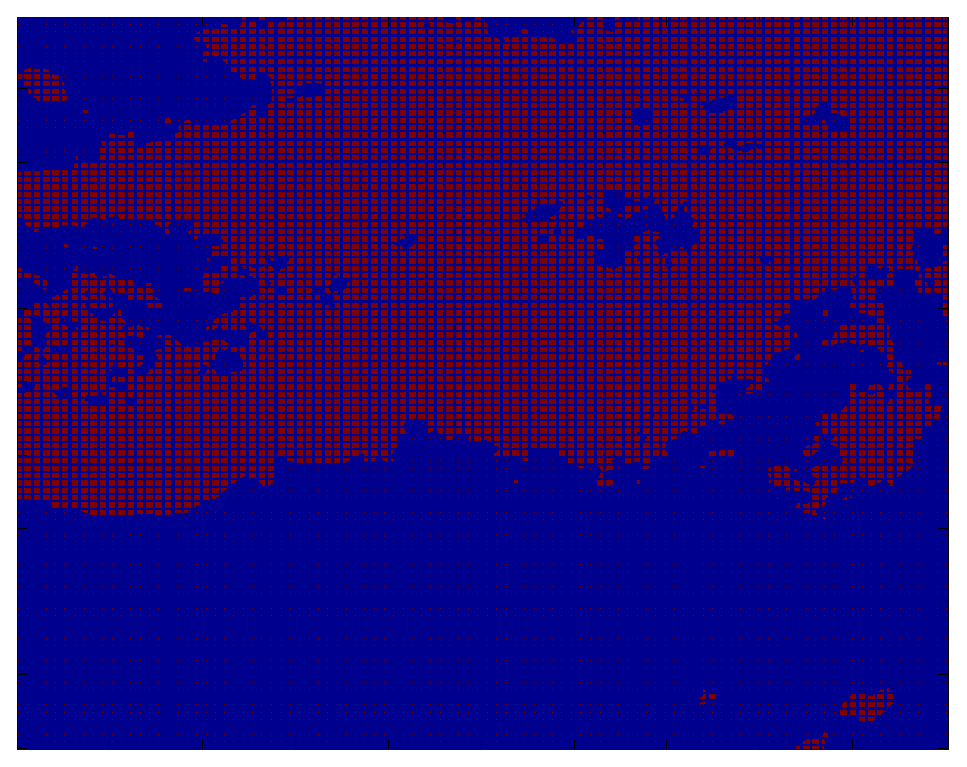
\includegraphics[scale=0.5]{images/fireBeginingIteration.eps}
\caption{Image after a few iterations}
\label{fig:setingfire}
\end{figure}

\begin{figure}
\center
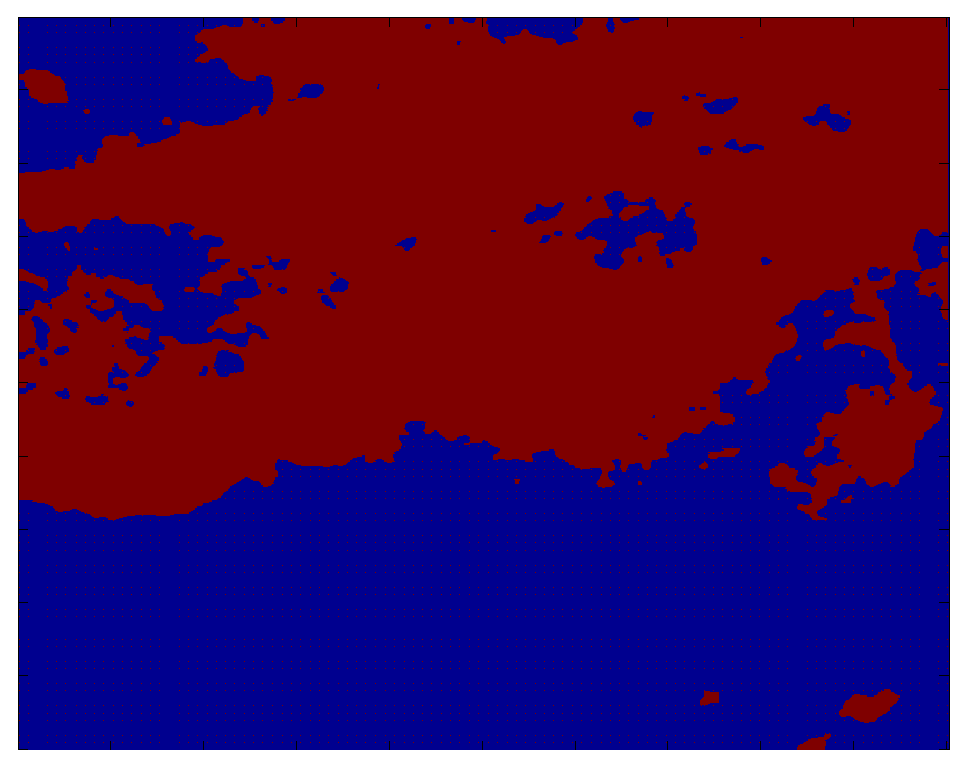
\includegraphics[scale=0.5]{images/firesresultNEW.eps}
\caption{Result of forest fire modelling after 40 iterations}
\label{fig:firesresult}
\end{figure}

The example output of this process is showed in Table \ref{Tab:Tablefireresult}.

\begin{table}
\caption{Result of forest fire modelling.}
{
\begin{tabular}{@{}ll}
\hline
\hspace{10 mm} $q_{i}$  \hspace{10 mm}&  \hspace{10 mm} $d_{i}$ \hspace{10 mm} \\
\hline
\hspace{10 mm} 0.1 \hspace{10 mm} & \hspace{10 mm} 31 \hspace{10 mm} \\
\hspace{10 mm} 0.2 \hspace{10 mm} & \hspace{10 mm} 40 \hspace{10 mm} \\
\hspace{10 mm} 0.3 \hspace{10 mm} & \hspace{10 mm} 31 \hspace{10 mm} \\
\hspace{10 mm} 0.4 \hspace{10 mm} & \hspace{10 mm} 30 \hspace{10 mm} \\
\hspace{10 mm} 0.5 \hspace{10 mm} & \hspace{10 mm} 40 \hspace{10 mm} \\
\hspace{10 mm} 0.6 \hspace{10 mm} & \hspace{10 mm} 24 \hspace{10 mm} \\
\hspace{10 mm} 0.7 \hspace{10 mm} & \hspace{10 mm} 29 \hspace{10 mm} \\
\hspace{10 mm} 0.8 \hspace{10 mm} & \hspace{10 mm} 27 \hspace{10 mm} \\
\hspace{10 mm} 0.9 \hspace{10 mm} & \hspace{10 mm} 22 \hspace{10 mm} \\
\cr
\hline
\end{tabular}
}
\label{Tab:Tablefireresult}
\end{table}

On the basis of intermediate calculations values, the example has been presented in Table \ref{Tab:Tablefireresult}, we can introduce the following formula for a potential feature:

\begin{equation}
q_{w}=\frac{\sum_{i=1}^{9}q_{i}d_{i}}{\sum_{i=1}^{9}d_{i}}
\label{eqfirefeatgure}
\end{equation}

The above equation can be applied to two thresholding comparison for signs: $\geq$ and $\leq$. Hence we have obtained 2 potential features with the use of above equation.

\subsection{Potential 4 features from the gray-level co-occurrence matrix and other statistics}
Four features have been generated using gray-level co-occurrence matrix (GLCM) from a given image. GLCM calculates how often a pixel with the gray-level (grayscale intensity) value i occurs horizontally adjacent to a pixel with the value j. Based on the GLCM approach,  4 potential features have been generated and presented in Table \ref{Tab:GLCM}:

\begin{table}
\caption{Definition of 4 features from histogram of co-occurring greyscale (GLCM) }
{
\begin{tabular}{@{}ll}
\hline
Name  &  Description  \\
\hline
Contrast & measure of the intensity contrast between a pixel and its neighbour over the whole image \\
\cr
Correlation & measure of how correlated a pixel is to its neighbour over the whole image \\
\cr
Energy & sum of squared elements in the GLCM \\
\cr
Homogeneity & value that measures the closeness of the distribution of elements in the GLCM to the GLCM diagonal \\
\hline
\end{tabular}
}
\label{Tab:GLCM}
\end{table}


\subsection{Potential 9 features based on box-counting fractal dimension}

The box-counting fractal dimension is a measure characterizing the fractal complexity. It is the particular case of the Mandelbrot fractal dimension, based on the notion of self-similarity of the structure at different scales. It measures how the length of the complex curve changes when the measurement is performed with the increased accuracy \citep{Schroeder2006}.
To characterize any curve, this curve is covered with the set of regular squared areas of the size $\varepsilon$. Thus, we have to calculate the number of squared areas containing any part of the given curve. Then number of found areas is denoted as N($\varepsilon$) (Formula \ref{eqboxcounting}). In our approach, we have used 9 boxes.

\begin{equation}
d=\lim_{\varepsilon\rightarrow\infty}\frac{log(N(\varepsilon))}{log(\varepsilon)}
\label{eqboxcounting}
\end{equation}

\subsection{36 features on the basis of Segmentation-based fractal texture analysis}

This approach allows us to generate 36 texture features on the basis of SFTA	algorithm (Segmentation-based Fractal Texture Analysis) and returns 16 vector D extracted from the input grayscale image. When we apply 6th fractal order, we can obtain 36 texture features.
The SFTA algorithm decomposes images into various thresholded images using several sets of lower and upper threshold values. The implementation has been based on Costa approach \citep{Costa2012}. Thresholded images are used to extract the fractal dimension. Since images with more jagged edges and prominent color differences tend to have higher fractal dimension, images with more uniform texture properties will have closer fractal dimension.

\subsection{16 features based on 4-level wavelet packet decomposition}

In this approach, the authors have applied db10 wavelet family. After wavelet packet decomposition, the portion of energy for every terminal node has been calculated based on the following equation (formula \ref{eqwaveletnodes}):

\begin{equation}
E=\Sigma_{k=1}^{N}|S_{jk}|^{2}
\label{eqwaveletnodes}
\end{equation}

where, $S_{jk}$ is an appropriate coefficient discrete wavelet transformation.

\section{Features selection}

To choose appropriate diagnostic features all 122 potentially available ones, best separating two classes of tissues (normal and abnormal), the authors have applied the method of sequential feature selection that, according to the author's practical knowledge, seems to create a suboptimal set of the most significant features from the perspective of breast cancer diagnostics. This approach selects a subset of features from the data matrix X that best predicts the data in y by sequentially selecting features until there is no improvement in prediction \citep{Matlab2015}. There is a possibility to apply a  chosen classifier (e.g. no-linear) for this selection method e.g SVM, random forest, decision tree. For every candidate feature subset, sequential feature selection performs 10-fold cross-validation by repeatedly calling function with different training subsets of X and y, XTRAIN and YTRAIN, and test subsets of X and y, XTEST and ytest. The result is  a logical vector indicating which features are finally chosen. After applying sequential features selection, we obtained 48 diagnostic features from 122 available ones.

\section{Experimental study}
In the experiments, we evaluated the performance of each proposed feature set for false-positive mammographic masses reduction. Furthermore, to highlight the importance of combining feature sets and feature selection steps, feature sets composed of all proposed descriptors (with and without feature selection) were considered.
 We have applied three types of classifiers: SVM, decision tree and random forest. For numerical experiments, the equal subset of normal and abnormal tissues trials have been chosen in randomize approach. The 10-fold stratified cross validation has been performed to compute the classification accuracy for each classifier.
 \subsection{Results}
Table \ref{Tab:ResultofSVM} summarizes the classification results achieved by the different proposed feature sets using  SVM, Decision tree and Random forest classifiers.


We can see that feature sets obtained through combination of all the descriptors (with and without feature selection) yield better results than each feature set used alone, regardless the  classification method that is used, which prove the usefulness of the combination step. Besides,  the feature selection step is very important since it increases the accuracy values for the three classifiers. Finally, the random forest achieves the highest accuracy ($= 81.09 \%$)), outperforming the SVM classifier ($= 80.01 \%$)) that is commonly used for mammographic masses classification.

\begin{table}
\caption{Accuracy (mean $\pm$ Standard deviation) of binary classification (normal vs. abnormal tissues) of mammography images using SVM, Decision tree and Random forest. }
{
\begin{tabular}{@{}llll}
\hline
Feature set  &  SVM&  Decision tree & Random forest\\
\hline
Gray level Co-occurrence matrix & 63.32\% $\pm$  2.43 & 63.19\% $\pm$   2.13& 64.66\% $\pm$  3.40\\
\cr
 Fractal analysis & 66.61\% $\pm$   2.79\%& 64.55\% $\pm$  2.23& 67.36\% $\pm$ 2.17\\
\cr
Hilbert image representation & 57.18\%$\pm$   2.15 & 58.18\% $\pm$  2.71& 61.88\% $\pm$  3.23\\
\cr
Kolmogorov-Smirnov descriptors & 55.87\% $\pm$    2.31& 55.66\% $\pm$   1.90& 58.22\% $\pm$  2.39\\
\cr
 Maximum sub-regions descriptors& 60.26\% $\pm$   2.13& 62.92\% $\pm$   2.71& 61.52\% $\pm$  2.63\\
\cr
 All descriptors (without feature selection)& 71.63\% $\pm$   0.96&70.11\% $\pm$  2.53& 71.42\% $\pm$  3.14\\
\cr
All descriptors (with feature selection) & 80.01\% $\pm$   5.05& 79.12\% $\pm$   5.51& 81.09\% $\pm$  4.51\\
\cr
%
\hline
\end{tabular}
}
\label{Tab:ResultofSVM}
\end{table}


\subsection{Comparison}
We compare our method to state-of-the-art curvelet-based mammogram characterization. Indeed, we have already used multiresolution texture analysis for mammogram characterization, and the proposed curvelet moments set outperforms state-of-the-art curvelet-based mammogram analysis methods \citep{Dhahbi2015}.  To further improve mammogram characterization, we investigate in this paper gray level mammogram features. Bearing in mind the superiority of multiresolution texture features over gray level texture features, we are not looking for a gray level mammogram description that outperforms multiresolution texture features, but rather it can be combined with them. Our findings show that the proposed feature set yields better results than several curvelet-based methods. Indeed, our highest accuracy result (Random Forest-81\%) is slightly better than biggest curvelet coefficients (BCC) (=80.65\% std 0.65\%), Statistical Curvelet Coefficients (SCC) (=80.01\% std 0.58 \%) and co-occurence matrix of curvelet coefficients (=80.69\% std 0.52\%). Our method is only outperformed by Curvelet Level Moments (CLM) (86.46\% std 0.91\%).
Motivated by the encouraging results obtained by the proposed gray level texture features as well as curvelet moments, our future work will include combination of such features to further improve mammogram characterization.

\begin{table}
\caption{Accuracy (mean $\pm$ Standard deviation) comparison of the proposed method against state-of-the-art methods for  binary classification (normal vs. abnormal tissues) of mammography images.}
{
\begin{tabular}{@{}ll}
\hline
Method  &  Accuracy  (mean $\pm$ Standard deviation) \\
\hline
Biggest curvelet coefficients & 80.65 \% $\pm$ 0.65  \\
\cr
Statistical curvelet coefficients & 80.01 \% $\pm$ 0.58  \\
\cr
Co-occurrence matrix of curvelet coefficients  & 80.69 \%$\pm$ 0.52  \\
\cr
Curvelet moments  & 86.46 \% $\pm$ 0.91 \\
\cr
Proposed method& 81 \% $\pm$ 4.5  \\

\hline
\end{tabular}
}
\label{Tab:Comparison}
\end{table}
\section{Conclusion}

In this paper, we have investigated several gray level texture analysis methods for mammogram characterization. The proposed methods include gray level co-occurrence matrix, fractal analysis, Hilbert’s image representation, Kolmogorov-Smirnov distance and maximum sub-region descriptors. By extracting features directly from the entire ROI, we not only escape the challenging problem of mammographic mass segmentation, but also we take into account  the texture surrounding the lesion, which is useful for breast cancer diagnosis \citep{Karahaliou2008}. A feature selection step was also included to choose the optimal feature set. Several classifiers (Random Forest, Support Vector Machine and Decision Tree) were considered to distinguish between normal tissues and masses.  Empirical evaluation in a large database composed of challenging suspicious regions extracted from the DDSM database prove the efficiency of the suggested method for false-positive reduction in mammographic mass detection.

\begin{thebibliography}{1}

\bibitem[Costa (2012)]{Costa2012}
Costa~A, Humpire-Mamani~G, Traina~A. 2012. An efficient algorithm for fractal analysis of textures. 2012 25th SIBGRAPI Conference on Graphics, Patterns and Images, 39–46, 2012.

\bibitem[Dhahbi et al.(2015)]{Dhahbi2015}
Dhahbi~S, Barhoumi~W, Zagrouba~E. 2015. Breast cancer diagnosis in digitized mammograms using curvelet moments, Comp. Biol. Med. 64 (2015) 79-90.

\bibitem[Ferlay et al.(2012)]{Ferlay2012}
Ferlay~J., Soerjomataram~I., Dikshit~R., Eser~S., Mathers~C., Rebelo~M., Bray~F. (2012). Cancer incidence and mortality worldwide: sources, methods and major patterns in GLOBOCAN 2012. International journal of cancer, 136(5), E359-E386.

\bibitem[Hofvind et al. (2009)]{Hofvind2009}
Hofvind~S, Ursin~G, Tretli~S, Sebuodegard~S, Moller~B. 2013. Breast cancer mor-tality in participants of the norwegian breast cancer screening program, Cancer 119 (2013) 3106–3112.

\bibitem[Heath et al. (1998)]{Heath1998}
Heath~M, Bowyer~K, Kopans~D, Kegelmeyer~W, Moore~R, Chang~K, Munishkumaran~S. 1998. Current status of the digital database for screening mammography, in Digital Mammography, Springer Netherlands (1998) 457–460.

\bibitem[Hussain (1998)]{Hussain2014}
Hussain, M. (2014). False-positive reduction in mammography using multiscale spatial Weber law descriptor and support vector machines. Neural Computing and Applications, 25(1), 83-93.

\bibitem[Jiang et al. (2015)]{Jiang2015}
Jiang~M, Zhang~S, Li~H, Metaxas~N. 2015. Computer-aided diagnosis of mammographic masses using scalable image retrieval, IEEE Transactions on Biomedical Engineering 62(2) (2015) 783–792.

\bibitem[Jotwani and Gralow (2009)]{Jotwani2009}
Jotwani~A, Gralow~J. 2009. Early detection of breast cancer, Mol. Diagnosis and Ther. 13(6) (2009) 349–357.

\bibitem[Junior et al. (2013)]{Junior2013}
Junior~G., Da Rocha~S. , Gattass~M., Silva~A., De Paiva~A (2013). A mass classification using spatial diversity approaches in mammography images for false positive reduction. Expert systems with applications, 40(18), 7534-7543.

\bibitem[Karahaliou et al. (2008)]{Karahaliou2008}
Karahaliou, A. N., Boniatis, I. S., Skiadopoulos, S. G., Sakellaropoulos, F. N., Arikidis, N. S., Likaki, E. A.,  Costaridou, L. I. (2008). Breast cancer diagnosis: analyzing texture of tissue surrounding microcalcifications. Information Technology in Biomedicine, IEEE Transactions on, 12(6), 731-738.

\bibitem[Kruk et al. (2015)]{Kruk2015}
Kruk~M, Swiderski~B, Osowski~S, Kurek~J, Slowinska~M, Walecka~I
Melanoma recognition using extended set of descriptors and classifiers, EURASIP Journal on Image and Video Processing, 2015,1,43,DOI: 10.1186/s13640-015-0099-9

\bibitem[Li et al. (2015)]{Li2015}
Li~Y., Chen~H., Yang~Y., Cheng~L., and Cao~L. (2015). A bilateral analysis scheme for false positive
reduction in mammogram mass detection. Computers in biology and medicine, 57, 84-95.

\bibitem[Liu et al. (2015)]{Liu2015}
Liu~X., Zeng~Z. (2015). A new automatic mass detection method for breast cancer with false positive reduction. Neurocomputing, 152, 388-402.

\bibitem[Matlab (2015)]{Matlab2015}
MathWorks, Inc. 2015. Matlab user manual, MathWorks, Natick, 2015

\bibitem[Nelson et al. (2009)]{Nelson2009}
Nelson~H, Tyne~K, Naik~A, Bougatsos~C, Chan~B, Nygren~P, Humphrey~L. 2009. Screening for breast cancer: Systematic evidence review update for the U. S. preventive services task force, Ann. Intern. Med. 151(10) (2009) 727–W242.

\bibitem[Swiderski (2015)]{Swiderski2015}
Swiderski~B, Osowski~S, Kruk~M, Kurek~J. 2015. Texture characterization based on the Kolmogorov-Smirnov distance, Expert Systems with Applications 42(1) (2015) 503–509

\bibitem[Schroeder (2006)]{Schroeder2006}
Schroeder~M., Fractals, Chaos, Power La-ws, 6 Ed. New York: W.H. Freeman and Company, 2006.

\bibitem[Tan (2014)]{Tan2014}
Tan~M., Pu~J., Zheng~B. (2014). Reduction of false-positive recalls using a computer-ized mammographic image feature analysis scheme. Physics in medicine and biology, 59(15), 4357.

\bibitem[WHO (2015)]{WHO2015}
World Health Organization. Breast cancer: prevention and control. WHO 2015.

\bibitem[Zyout (2015)]{Zyout2015}
Zyout~I., Czajkowska~J., Grzegorzek~M. (2015). Multi-scale textural feature extraction and particle swarm optimization based model selection for false positive reduction in mammography. Computerized Medical Imaging and Graphics, 46, 95-107.

\bibitem[Vallez (2014)]{Vallez2014}
Vállez, N., Bueno, G., Déniz, O., Dorado, J., Seoane, J. A., Pazos, A., Pastor, C. (2014). Breast density classification to reduce false positives in CADe systems. Computer methods and programs in biomedicine, 113(2), 569-584.

\bibitem[Sampaio (2015)]{Sampaio2015}
de Sampaio, W. B., Silva, A. C., de Paiva, A. C.,  Gattass, M. (2015). Detection of masses in mammograms with adaption to breast density using genetic algorithm, phylogenetic trees, LBP and SVM. Expert Systems with Applications, 42(22), 8911-8928.

\bibitem[Liu (2014)]{Liu2014}
Liu, J., Zhang, S., Liu, W., Zhang, X.,  Metaxas, D. N. (2014, April). Scalable mammogram retrieval using anchor graph hashing. In 2014 IEEE 11th International Symposium on Biomedical Imaging (ISBI) (pp. 898-901). IEEE.
\end{thebibliography}


\end{document}

%%
